% !TEX program = pdflatex
\documentclass[conference]{IEEEtran}
\IEEEoverridecommandlockouts

\usepackage{amsmath,amssymb,amsfonts}
\usepackage{graphicx}
\usepackage{booktabs}
\usepackage{cite}
\usepackage[colorlinks=false,urlcolor=black,linkcolor=black,citecolor=black]{hyperref}

\newcommand{\R}{\mathbb{R}}
\newcommand{\triu}{\operatorname{triu}}
\newcommand{\simcos}{\operatorname{sim}_{\mathrm{cos}}}
\newcommand{\tr}{\operatorname{tr}}

\begin{document}

\title{When Physiological Plausibility Misleads:\\ Covariance-Aligned Quality Gates for Synthetic Motor-Imagery EEG}

\author{
\IEEEauthorblockN{Anonymous Authors}
\IEEEauthorblockA{\textit{Anonymous Institution}\\
\textit{City, Country}\\
author@example.com}
}

\maketitle

\begin{abstract}
Generative models are increasingly used to augment scarce motor-imagery (MI)
electroencephalography (EEG) datasets. Their synthetic samples are commonly
filtered by \emph{physiological} quality gates, such as the event-related
desynchronization (ERD) a motor-imagery trial is expected to produce. We show
that this premise does not hold: an ERD gate measures a \emph{temporal} energy
contrast, while the downstream common-spatial-pattern (CSP) classifier consumes
the \emph{spatial} covariance of each trial. The two criteria occupy distinct
representational spaces, so an ERD gate can be blind to harmful corruption and
itself damaging. We propose a dual gate that operates in the decoder's own
covariance feature space. A plausibility gate scores the cosine similarity of a
trial's covariance to its class template; a discriminative gate checks the Fisher
linear-discriminant projection gap. On a real state-of-the-art generative
model---DDF-Net, a denoising-diffusion model whose per-channel synthesis
collapses cross-channel covariance (synthetic cosine similarity $0.368$ versus
real $0.996$)---unfiltered samples drop CSP accuracy from $0.833$ to $0.667$.
Our dual gate admits $0/144$ samples ($0\%$ leakage) and restores the $0.833$
baseline with no loss. These results argue that generative EEG models must model
the channel distribution jointly, and that a gate is effective only when it
shares the decoder's representation.
\end{abstract}

\begin{IEEEkeywords}
EEG, motor imagery, synthetic data, generative models, diffusion, common
spatial patterns, data quality.
\end{IEEEkeywords}

\section{Introduction}
\label{sec:intro}

Decoding motor imagery from EEG underpins non-invasive brain--computer
interfaces (BCIs), but the scarcity and high inter-subject variability of
labeled trials limit the performance of data-hungry decoders
\cite{blankertz2008optimizing,schirrmeister2017deep,lawhern2018eegnet,fahimi2019inter}. To relieve
this bottleneck, researchers increasingly synthesize artificial MI-EEG with
generative models---generative adversarial networks (GANs), variational
autoencoders (VAEs), and, most recently, denoising diffusion probabilistic
models (DDPMs)---and use the samples to augment training
\cite{goodfellow2014generative,kingma2014auto,ho2020denoising,dhariwal2021diffusion,
song2021score,hartmann2018eeg,lashgari2020data,vetter2024generating,dere2025motor,li2026diffusion}.

Because generated samples can be poor, a natural practice is to gate them by a
\emph{physiological} criterion before mixing them into the training set. In MI
the dominant such criterion is the event-related desynchronization (ERD): a
real motor-imagery trial should exhibit a band-power decrease over the
contralateral sensorimotor cortex during the task
\cite{pfurtscheller1999event}. This paper interrogates the unstated assumption
behind that practice---that a \emph{physiologically plausible} sample is
necessarily a \emph{useful} sample for the downstream decoder---and shows that
the assumption does not hold.

The root cause is a representational mismatch. ERD is a \emph{temporal}
quantity: a ratio of band power between a baseline and a task window. The
dominant MI decoder, CSP followed by a linear discriminant
\cite{ramoser2000optimal,blankertz2008optimizing,lotte2018review}, consumes a
\emph{spatial} quantity: the per-trial channel covariance matrix
$\mathbf{X}\mathbf{X}^{\top}$. A gate built on the former is therefore, in
principle, blind to exactly the structure the latter exploits, and vice versa.
We demonstrate three concrete consequences on controlled corruption. An ERD gate
cannot detect white-noise corruption that destroys the covariance off-diagonal;
it spuriously deletes harmless time-shifted trials; and in a full-data regime it
can itself reduce accuracy. A covariance-aligned gate, in contrast, rejects the
corruption while preserving the harmless perturbation.

Our contributions are threefold:
\begin{enumerate}
  \item We identify and quantify the negative result that a physiological ERD
        gate is misaligned with the covariance representation of the CSP
        decoder, and can be both ineffective and harmful (Section~\ref{sec:method},
        Section~\ref{sec:results}).
  \item We propose a \emph{dual covariance-aligned gate} operating on the exact
        feature space of the downstream decoder: a plausibility gate using
        cosine similarity to the class covariance template, and a discriminative
        gate using the Fisher linear-discriminant projection gap
        (Section~\ref{sec:method}).
  \item We validate the gate against a real state-of-the-art generative
        model---DDF-Net, a diffusion-based MI generator---and show that its
        per-channel synthesis collapses spatial covariance, that unfiltered
        samples are actively harmful, and that our gate achieves $0\%$ leakage
        while restoring baseline accuracy with no loss (Section~\ref{sec:results},
        Section~\ref{sec:discussion}).
\end{enumerate}

\section{Method}
\label{sec:method}

\subsection{Problem setting and downstream decoder}
\label{sec:setting}

We consider labeled MI-EEG trials $(\mathbf{X}_i, y_i)$, where
$\mathbf{X}_i\in\R^{C\times T}$ is a trial with $C=22$ EEG channels and $T$ time
samples, and $y_i\in\{-1,+1\}$ denotes left- versus right-hand imagery. The
downstream decoder is a two-stage CSP + linear-discriminant-analysis (LDA)
pipeline \cite{ramoser2000optimal,blankertz2008optimizing}. CSP computes spatial
filters from the per-class mean \emph{spatial covariance} matrices; that is, the
decoder's only contact with a trial is through
\begin{equation}
  \mathbf{C}_i \;=\; \mathbf{X}_i\,\mathbf{X}_i^{\top}\;\in\R^{C\times C},
  \label{eq:cov}
\end{equation}
the uncentered energy covariance. Any quality gate that is to remain faithful to
the decoder must therefore judge trials in the same covariance space.

We reduce $\mathbf{C}_i$ to a scale-invariant feature vector by trace
normalization followed by vectorization of the upper triangle (including the
diagonal),
\begin{equation}
  \boldsymbol{\phi}_i \;=\; \triu\!\Big(\frac{\mathbf{C}_i}{\tr(\mathbf{C}_i)}\Big)
  \;\in\;\R^{d},
  \qquad d = C(C+1)/2 = 253,
  \label{eq:feat}
\end{equation}
which matches the affine-invariance step of Riemannian covariance alignment and
isolates cross-channel structure from overall trial power. We utilize this
Euclidean vectorization for computational efficiency; while Riemannian distances
are theoretically rigorous, cosine similarity on trace-normalized vectors
provides a lightweight yet highly discriminative proxy for real-time gating.

\subsection{Gate 1: covariance plausibility}
\label{sec:gate1}

The first gate tests whether a trial \emph{looks like} plausible EEG of its
class. From the real calibration set we form a per-class covariance template
$\boldsymbol{\mu}_c = \mathbb{E}[\boldsymbol{\phi}\mid y=c]$ and score each
trial by the cosine similarity of its covariance features to its own class
template,
\begin{equation}
  \simcos(\boldsymbol{\phi}, \boldsymbol{\mu}_c)
  \;=\;
  \frac{\boldsymbol{\phi}\cdot\boldsymbol{\mu}_c}
       {\lVert\boldsymbol{\phi}\rVert\,\lVert\boldsymbol{\mu}_c\rVert}.
  \label{eq:cosine}
\end{equation}
We calibrate an acceptance window as the 5th--95th percentile of the
within-class similarity distribution of real trials,
$\mathcal{A}_c=\big[Q_5(\{s_i\}_{y_i=c}),\;Q_{95}(\{s_i\}_{y_i=c})\big]$, and a
trial is retained iff $\simcos(\boldsymbol{\phi}_i,\boldsymbol{\mu}_{y_i})\in
\mathcal{A}_{y_i}$. Because white-noise corruption inflates the diagonal
(self-power) relative to the off-diagonal (cross-channel) entries, it rotates
$\boldsymbol{\phi}$ away from $\boldsymbol{\mu}_c$ and drives the similarity out
of the window. Notably, a class-ambiguous blend of a left and a right
trial is still a \emph{valid} covariance and passes Gate~1; this motivates a
second, discriminative gate.

\subsection{Gate 2: discriminative projection gap}
\label{sec:gate2}

The second gate tests whether a trial carries the \emph{correct class}
information. We fit a Fisher LDA on the covariance features of real trials,
obtaining a discriminative direction $\mathbf{w}\in\R^{d}$ (with a small ridge
regularization) that best separates the two classes
\cite{fisher1936use}. A trial is projected to a scalar score
\begin{equation}
  z_i \;=\; \boldsymbol{\phi}_i^{\top}\mathbf{w},
  \label{eq:score}
\end{equation}
and we calibrate per-class acceptance windows
$\mathcal{D}_c=\big[Q_5(\{z_j\}_{y_j=c}),\,Q_{95}(\{z_j\}_{y_j=c})\big]$ on
real trials. A trial is retained iff $z_i\in\mathcal{D}_{y_i}$.
For real MI data the two class score distributions are well separated with an
intermediate \emph{rejection gap}: a class-mixed trial, being an average of the
two class covariances, projects near the midpoint between the class modes and
lands in the gap, where it is rejected by both windows. The dual gate admits a
trial only if it passes Gate~1 \emph{and} Gate~2.

\section{Experiments}
\label{sec:experiments}

\subsection{Dataset and protocol}
\label{sec:data}

We use the BCI Competition IV dataset 2a, which records $22$ EEG channels at
$250$\,Hz from $9$ subjects (A01--A09) performing four-class MI
\cite{tangermann2012review,brunner2008bci}. We restrict to the left- and
right-hand classes. We calibrate the gates on subject A01's training session
(A01T) with a fixed $108/36$ trial split, and evaluate downstream accuracy over
$10$ seeds; synthetic batches contain $144$ trials ($72$ per class,
balanced).

\subsection{Controlled corruption modes}
\label{sec:modes}

To probe the gates under known, interpretable defects, we generate three
synthetic-batch families from real A01T trials: \textbf{Mode~1} (class
mixing), averaging one left and one right trial, producing a valid but
class-ambiguous covariance; \textbf{Mode~2} (white noise), adding $0$\,dB
Gaussian noise, which attenuates cross-channel structure while inflating the
diagonal; and \textbf{Mode~3} (time shift), a circular temporal shift, which
preserves the covariance and is harmless to CSP.

\subsection{Real generative model: DDF-Net}
\label{sec:ddfnet}

As a terminal test we use DDF-Net, a diffusion-based MI-EEG model that augments
a dual-domain classification network with DDPM-generated samples
\cite{li2026diffusion}. We train its Stage-1 DDPM (a UNet-style architecture
with $T=100$ diffusion steps and $38.93$\,M parameters) on A01T and sample
$144$ synthetic trials. Our goal is not to benchmark DDF-Net's state-of-the-art
generative performance, but to use it as a representative generative
architecture that exposes the structural vulnerability of per-channel synthesis.
Because the generator models each of the channels
\emph{independently} and reassembles them into a trial afterwards, the joint
cross-channel distribution is never learned---an ideal stress test for a
covariance gate.

\section{Results}
\label{sec:results}

\subsection{The gate is selective on controlled corruption}
\label{sec:results-controlled}

The dual gate behaves exactly as designed. On the A01T synthetic batch, Gate~1
rejects $0/144$ white-noise trials (Mode~2) but retains $123/144$ class-mixed
trials (Mode~1), which are still valid covariances; Gate~2 then rejects the
class-ambiguous blends, reducing Mode-1 retention to $50/144$. For time-shifted
trials (Mode~3), whose covariance is unchanged, the dual gate correctly retains
$114/144$, i.e., it does not spuriously kill a harmless perturbation. By
contrast, an ERD gate retains $106/144$ of the white-noise trials while deleting
roughly $20\%$ of the harmless time-shifted trials.

Table~\ref{tab:nine} reports aggregate downstream accuracy across the $9$
subjects at the most severe ($100\%$) contamination level. On white noise
(Mode~2), unfiltered augmentation drops accuracy from $0.762$ to $0.690$
(paired $t$-test $p<0.001$), and the covariance-aligned gates restore it to
$0.762$, matching baseline. On class mixing (Mode~1) the dual gate partially recovers
the performance loss at lower contamination levels ($p=0.016$ at $25\%$,
$p=0.014$ at $50\%$); at $100\%$ contamination the improvement is not
significant ($p=0.524$), consistent with a ceiling effect when abundant real
data remain. Time shifts (Mode~3) induce no systematic degradation.

\begin{table}[!t]
\caption{Aggregate downstream accuracy (mean $\pm$ std over $9$ subjects) at
$100\%$ contamination. Mode 1: class mixing; Mode 2: white noise; Mode 3: time
shift. ``Cov'' and ``Dual'' denote the covariance-only gate (Gate~1) and the
dual gate (Gates 1+2).}
\label{tab:nine}
\centering
\setlength{\tabcolsep}{4pt}
\begin{tabular}{@{}l c c c c@{}}
\toprule
Mode & Base & Unf. & Cov & Dual \\
\midrule
1 (mix)   & $0.762{\pm}0.125$ & $0.732{\pm}0.117$ & $0.737{\pm}0.112$ & $0.739{\pm}0.128$ \\
2 (noise) & $0.762{\pm}0.125$ & $0.690{\pm}0.156$ & $0.762{\pm}0.125$ & $0.762{\pm}0.125$ \\
3 (shift) & $0.762{\pm}0.125$ & $0.740{\pm}0.126$ & $0.743{\pm}0.128$ & $0.744{\pm}0.130$ \\
\bottomrule
\end{tabular}
\end{table}

\begin{figure}[!t]
\centering
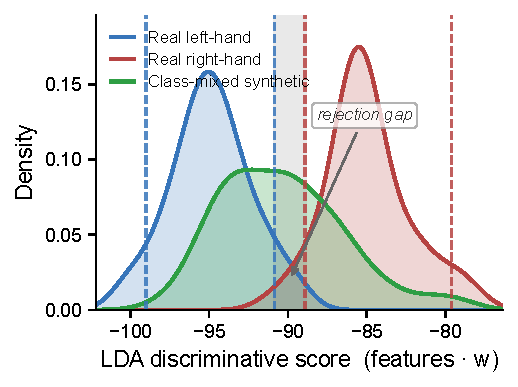
\includegraphics[width=\linewidth]{figures/fig_projection_gap.pdf}
\caption{Fisher LDA discriminative scores of real left- and right-hand trials
(blue/red) and class-mixed synthetic trials (green). The two classes' $5\%$--$95\%$
acceptance windows are separated by a shaded \emph{rejection gap}; class-ambiguous
blends project near the midpoint and fall into this gap, where Gate~2 rejects
them.}
\label{fig:gap}
\end{figure}

\subsection{Real-model validation: DDF-Net collapses covariance}
\label{sec:results-ddfnet}

Against the real DDF-Net generator the gate is decisive. Fig.~\ref{fig:cov}
visualizes the root cause: the trace-normalized mean covariance of DDF-Net
synthetic right-hand trials is nearly diagonal, whereas real trials carry
substantial off-diagonal (cross-channel) structure; the difference map isolates
exactly the structure that per-channel generation discards. Fig.~\ref{fig:cos}
translates this into the gate's decision variable: real trials concentrate at
cosine similarity $0.996$ to their class template, while synthetic trials
cluster at $0.368$---well below the $[0.990,\,0.999]$ acceptance window, so
$144/144$ synthetic trials fall outside and are rejected ($0\%$ leakage).

Table~\ref{tab:ddfnet} reports the terminal result. Feeding all $144$ unfiltered
synthetic trials into training degrades CSP accuracy from $0.8333$ to $0.6667$,
a $0.17$ drop that confirms the synthetic data are not merely uninformative but
actively harmful. Applying the covariance gate (or the full dual gate) keeps
$0/144$ samples and restores accuracy to the $0.8333$ baseline with no loss.

\begin{figure*}[!t]
\centering
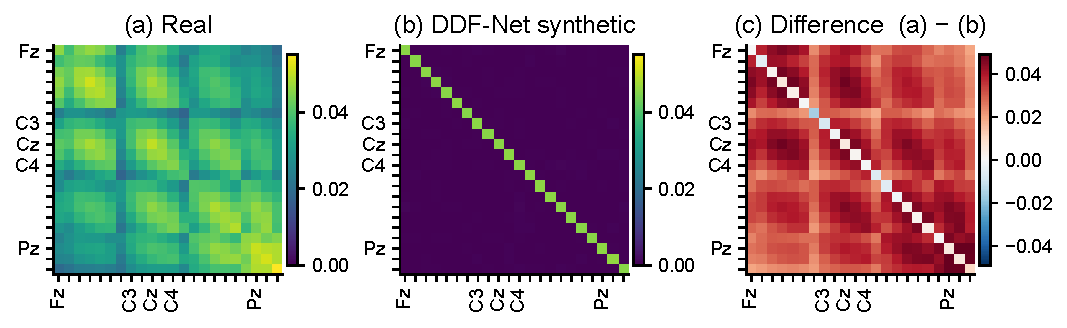
\includegraphics[width=\textwidth]{figures/fig_covariance_collapse.pdf}
\caption{Trace-normalized mean spatial covariance ($22\times22$) of
(a) real right-hand trials, (b) DDF-Net synthetic right-hand trials, and
(c) their element-wise difference. Per-channel independent generation produces a
near-diagonal synthetic covariance, discarding the off-diagonal (cross-channel)
structure on which CSP spatial filters depend.}
\label{fig:cov}
\end{figure*}

\begin{figure}[!t]
\centering
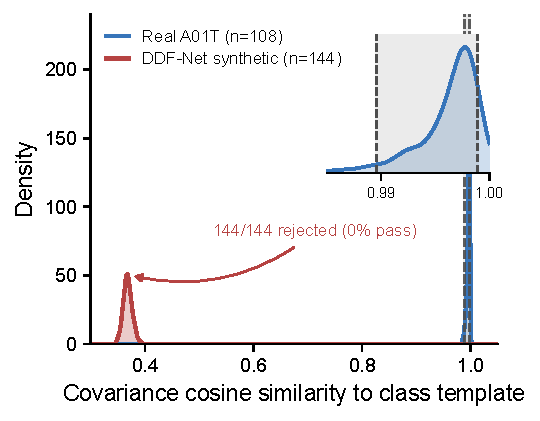
\includegraphics[width=\linewidth]{figures/fig_cos_sim_rejection.pdf}
\caption{Distributions of per-trial covariance cosine similarity to the class
template for real A01T trials (blue) and the $144$ DDF-Net synthetic trials
(red), with the $5\%$--$95\%$ acceptance window shaded. Synthetic similarity
(mean $0.368$) collapses far below the window $[0.990,\,0.999]$; all $144$
trials fall outside, so Gate~1 rejects $100\%$. (inset: zoom on the acceptance window).}
\label{fig:cos}
\end{figure}

\begin{table}[!t]
\caption{Downstream CSP accuracy on DDF-Net synthetic augmentation. ``Kept''
is the number of synthetic trials admitted into training.}
\label{tab:ddfnet}
\centering
\begin{tabular}{l c c}
\toprule
Condition & Accuracy & Kept \\
\midrule
Baseline (no augmentation) & $0.8333$ & -- \\
Unfiltered                 & $0.6667$ & $144/144$ \\
Covariance gate (Gate~1)   & $0.8333$ & $0/144$ \\
Dual gate (Gates 1+2)      & $0.8333$ & $0/144$ \\
\bottomrule
\end{tabular}
\end{table}

\section{Discussion}
\label{sec:discussion}

\subsection{Why per-channel generation is harmful}
\label{sec:why}

CSP is a spatial method: its filters are the eigenvectors of a generalized
eigenvalue problem formed from per-class \emph{covariance} matrices
\cite{ramoser2000optimal,blankertz2008optimizing}. A generator that synthesizes
each channel independently and stitches channels together afterwards can
reproduce each channel's marginal power spectrum, but it cannot reproduce the
cross-channel correlations that constitute the spatial structure CSP exploits.
The result is the diagonalization visible in Fig.~\ref{fig:cov}: the synthetic
trials occupy a region of covariance space so far from the real class templates
(cosine similarity $0.368$ versus $0.996$) that even a coarse plausibility gate
rejects them all. This is a stronger statement than ``the samples are noisy''
---it shows that a \emph{per-channel} generative model is architecturally
incapable of producing CSP-useful data, regardless of how realistic its
single-channel signals appear. We therefore argue that generative EEG models
intended for spatial decoders must model the \emph{joint} channel distribution.

\subsection{Why the representation must match the decoder}
\label{sec:repr}

The negative result on the ERD gate follows the same logic in reverse. ERD is a
temporal band-power contrast; it is decoupled from the spatial covariance the
decoder reads. As a result, an ERD gate is blind to covariance collapse and can
simultaneously reject harmless temporal perturbations. Our dual gate sidesteps
this by construction: both of its decision variables---cosine similarity and the
LDA projection---are computed on the identical trace-normalized covariance
features that the decoder consumes. The alignment, not the specific threshold,
is what makes the gate effective, and we expect the principle to transfer to any
decoder whose representation can be made explicit. Although we demonstrate with
CSP, the core principle---aligning the gate's representation with the decoder's
receptive field---generalizes to any explicit spatial decoder (e.g., EEGNet).

\subsection{Limitations}
\label{sec:limitations}

Three limitations bound our conclusions. First, a ceiling effect: when real data
are abundant (e.g., Mode~1 at $100\%$ contamination), the marginal value of the
gate disappears, so significance is expected to vanish. Second, boundary leakage:
class-mixed discriminative scores follow a distribution centered near the class
boundary, so a fraction of Mode-1 blends still land inside a class window
($50/144$ retained); this is the inherent cost of a percentile window, and
tightening it would misclassify the harmless Mode-3 trials. Third, we calibrate
the gate on a single subject and session (A01T), so cross-subject and
cross-session generalization remains open. Future work will validate the
cross-subject transferability of the covariance templates.

\section{Conclusion}
\label{sec:conclusion}

We showed that physiological plausibility is an unreliable proxy for
downstream utility in synthetic MI-EEG: an ERD gate operates in a temporal space
decoupled from the spatial covariance that CSP decodes, and can be both blind to
harmful corruption and itself damaging. A dual gate aligned to the decoder's
covariance representation---cosine-similarity plausibility plus a
discriminative projection gap---recovers downstream accuracy under controlled
corruption and, against the real DDF-Net diffusion generator, achieves $0\%$
leakage ($0/144$) while restoring the $0.833$ baseline with no loss. The finding
that per-channel synthesis collapses spatial covariance carries a direct design
imperative: generative EEG models for spatial decoders must model the joint
channel distribution, and quality gates must share the decoder's representation
to serve as the last line of defense before deployment.

\bibliographystyle{IEEEtran}
\bibliography{references}

\end{document}
